\documentclass[notes,11pt, aspectratio=169, xcolor=table]{beamer}

\usepackage{pgfpages}
% These slides also contain speaker notes. You can print just the slides,
% just the notes, or both, depending on the setting below. Comment out the want
% you want.
\setbeameroption{hide notes} % Only slide
%\setbeameroption{show only notes} % Only notes
%\setbeameroption{show notes on second screen=right} % Both

\usepackage{helvet}
\usepackage[default]{lato}
\usepackage{array}
\usepackage[utf8]{inputenc} 

\newtheorem{proposition}{Proposition}

\usepackage{tikz}
\usetikzlibrary{shapes.geometric}
\usepackage{pgfplots}
\usepackage{graphicx}
\usepackage{verbatim}
\setbeamertemplate{note page}{\pagecolor{yellow!5}\insertnote}
\usetikzlibrary{positioning}
\usetikzlibrary{snakes}
\usetikzlibrary{calc}
\usetikzlibrary{arrows}
\usetikzlibrary{decorations.markings}
\usetikzlibrary{shapes.misc}
\usetikzlibrary{matrix,shapes,arrows,fit,tikzmark}
\usepackage{amsmath}
\usepackage{mathpazo}
\usepackage{hyperref}
\usepackage{lipsum}
\usepackage{multimedia}
\usepackage{graphicx}
\usepackage{multirow}
\usepackage{graphicx}
\usepackage{dcolumn}
\usepackage{bbm}
\usepackage[style=authoryear,sorting=nyt,uniquename=false]{biblatex}
\newcommand{\blue}[1]{\textcolor{blue}{#1}}
\newcommand{\white}[1]{\textcolor{white}{#1}}

\addbibresource{references.bib} 

\newcolumntype{d}[0]{D{.}{.}{5}}

\def\@@mybluebox[#1][#2]#3{
    \sbox\mytempbox{#3}%
    \mytemplen\ht\mytempbox
    \advance\mytemplen #1\relax
    \ht\mytempbox\mytemplen
    \mytemplen\dp\mytempbox
    \advance\mytemplen #2\relax
    \dp\mytempbox\mytemplen
    \colorbox{myblue}{\hspace{1em}\usebox{\mytempbox}\hspace{1em}}}


\usepackage{changepage}
\usepackage{appendixnumberbeamer}
\newcommand{\beginbackup}{
   \newcounter{framenumbervorappendix}
   \setcounter{framenumbervorappendix}{\value{framenumber}}
   \setbeamertemplate{footline}
   {
     \leavevmode%
     \hline
     box{%
       \begin{beamercolorbox}[wd=\paperwidth,ht=2.25ex,dp=1ex,right]{footlinecolor}%
%         \insertframenumber  \hspace*{2ex} 
       \end{beamercolorbox}}%
     \vskip0pt%
   }
 }
\newcommand{\backupend}{
   \addtocounter{framenumbervorappendix}{-\value{framenumber}}
   \addtocounter{framenumber}{\value{framenumbervorappendix}} 
}


\usepackage{graphicx}
\usepackage[space]{grffile}
\usepackage{booktabs}

% These are my colors -- there are many like them, but these ones are mine.
\definecolor{blue}{RGB}{0,114,178}
\definecolor{red}{RGB}{213,94,0}
\definecolor{yellow}{RGB}{240,228,66}
\definecolor{green}{RGB}{0,158,115}

\hypersetup{
  colorlinks=false,
  linkbordercolor = {white},
  linkcolor = {blue}
}


%% I use a beige off white for my background
\definecolor{MyBackground}{RGB}{255,253,218}

%% Uncomment this if you want to change the background color to something else
%\setbeamercolor{background canvas}{bg=MyBackground}

%% Change the bg color to adjust your transition slide background color!
\newenvironment{transitionframe}{
  \setbeamercolor{background canvas}{bg=yellow}
  \begin{frame}}{
    \end{frame}
}

\setbeamercolor{frametitle}{fg=blue}
\setbeamercolor{title}{fg=blue}
\setbeamertemplate{footline}[frame number]
\setbeamertemplate{navigation symbols}{} 
\setbeamertemplate{itemize items}{-}
\setbeamercolor{itemize item}{fg=blue}
\setbeamercolor{itemize subitem}{fg=blue}
\setbeamercolor{enumerate item}{fg=blue}
\setbeamercolor{enumerate subitem}{fg=blue}
\setbeamercolor{button}{bg=MyBackground,fg=blue,}



% If you like road maps, rather than having clutter at the top, have a roadmap show up at the end of each section 
% (and after your introduction)
% Uncomment this is if you want the roadmap!
% \AtBeginSection[]
% {
%    \begin{frame}
%        \frametitle{Roadmap of Talk}
%        \tableofcontents[currentsection]
%    \end{frame}
% }
\setbeamercolor{section in toc}{fg=blue}
\setbeamercolor{subsection in toc}{fg=red}
\setbeamersize{text margin left=1em,text margin right=1em} 

\newenvironment{wideitemize}{\itemize\addtolength{\itemsep}{10pt}}{\enditemize}

\usepackage{environ}
\NewEnviron{videoframe}[1]{
  \begin{frame}
    \vspace{-8pt}
    \begin{columns}[onlytextwidth, T] % align columns
      \begin{column}{.58\textwidth}
        \begin{minipage}[t][\textheight][t]
          {\dimexpr\textwidth}
          \vspace{8pt}
          \hspace{4pt} {\Large \sc \textcolor{blue}{#1}}
          \vspace{8pt}
          
          \BODY
        \end{minipage}
      \end{column}%
      \hfill%
      \begin{column}{.42\textwidth}
        \colorbox{green!20}{\begin{minipage}[t][1.2\textheight][t]
            {\dimexpr\textwidth}
            Face goes here
          \end{minipage}}
      \end{column}%
    \end{columns}
  \end{frame}
}

\title[]{International Trade: Lecture XX}
\subtitle[]{Diverse Firms and Trade: The Melitz Model}
\author[Góes]
{Carlos Góes\inst{1}}
\date{Fall 2025}
\institute[GWU]{\inst{1} George Washington University }



\begin{document}

%%% TIKZ STUFF
\tikzset{   
        every picture/.style={remember picture,baseline},
        every node/.style={anchor=base,align=center,outer sep=1.5pt},
        every path/.style={thick},
        }
\newcommand\marktopleft[1]{%
    \tikz[overlay,remember picture] 
        \node (marker-#1-a) at (-.3em,.3em) {};%
}
\newcommand\markbottomright[2]{%
    \tikz[overlay,remember picture] 
        \node (marker-#1-b) at (0em,0em) {};%
}
\tikzstyle{every picture}+=[remember picture] 
\tikzstyle{mybox} =[draw=black, very thick, rectangle, inner sep=10pt, inner ysep=20pt]
\tikzstyle{fancytitle} =[draw=black,fill=red, text=white]
%%%% END TIKZ STUFF



%----------------------------------------------------------------------%
%-------------------       TITLE PAGE       ---------------------------%
%----------------------------------------------------------------------%





%----------------------------------------------------------------------%






%----------------------------------------------------------------------%
%----------------------------------------------------------------------%

%----------------------------------------------------------------------%
\frame{\titlepage}
\addtocounter{framenumber}{-1}
%----------------------------------------------------------------------%

\section{Intro and recap}

\begin{frame}{Last class}

    \begin{wideitemize}
        \item We extended the Krugman framework to one with diverse firms
        \item Firms differ in their productivities, which means their marginal and average costs will be different
        \item With identical fixed costs, firms with different productivities optimize to different values
        \item More productive firms charge lower prices, sell higher quantities, have higher revenues and profits
    \end{wideitemize}
    
\end{frame}

\begin{frame}{This class}
    \begin{wideitemize}
    \item This is all consistent with the broad facts we saw about exporters
    \item We will learn how to solve for the equilibrium of this model (with charts, mostly)
    \item Minimum productivity threshold $\varphi_{\min}$ will emerge in equilibrium
    \item Equilibrium number of goods available $N^*$ will also emerge in equilibrium
    \item We will also see what happens when countries open up to trade
    \end{wideitemize}
\end{frame}

\begin{frame}{Diverse firms and monopolistic competition}
Firms producing different goods have different marginal costs...
\centering
    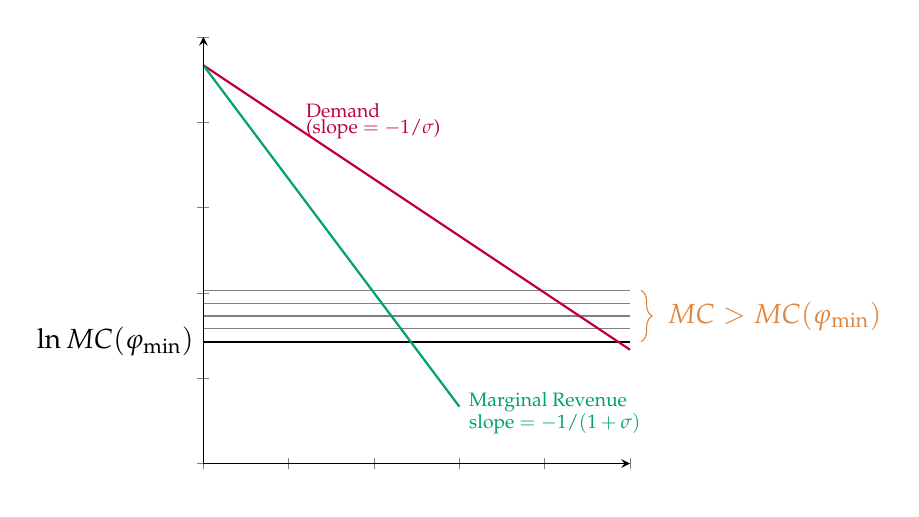
\begin{tikzpicture}
    \pgfmathsetmacro{\K}{7}
    \pgfmathsetmacro{\sigmaa}{1.5}

    \pgfmathsetmacro{\A}{7}
    \pgfmathsetmacro{\b}{0.75}
    \pgfmathsetmacro{\m}{0.35}
    \pgfmathsetmacro{\s}{2.25}
    \pgfmathsetmacro{\pmax}{\A/\b}          % choke price  (demand intercept)
    \pgfmathsetmacro{\qc}{\A - \b/\m}       % competitive quantity (P = MC)
        
    
    
    \begin{axis}[
        ymin=0, ymax=10,
        xmin=0, xmax=5,
        yticklabel=\empty,
        xticklabel=\empty,
        axis lines=left,
        enlargelimits=false,
        clip=false,
        axis on top,
        scaled x ticks=false,
        width=7cm, height=7cm,
        title style={font=\bfseries}
    ]

        
        \pgfmathsetmacro{\qs}{((\A / \b - (1/ \m  * \s) ) / ( 2/\b))}
        \pgfmathsetmacro{\ps}{ (\A / \b) - 1/\b * \qs }
        % revenue
        
        \addplot[gray, domain=0:5] {1/\m +.3};
        \addplot[gray, domain=0:5] {1/\m +.6};
        \addplot[gray, domain=0:5] {1/\m +.9};
        \addplot[gray, domain=0:5] {1/\m +1.2};

        \draw[decorate,decoration={brace,amplitude=4pt},xshift=4pt,red!75]
            (axis cs:5,1/\m +1.2) -- (axis cs:5,1/\m)
            node[midway,right=6pt]{$MC > MC(\varphi_{\min})$};

        
        
        \pgfmathsetmacro{\q}{((\A / \b - 1/ \m ) / ( 2/\b))}
        \pgfmathsetmacro{\p}{ (\A / \b) - 1/\b * \q }
        % revenue
        \addplot[black, thick, domain=0:5] {1/\m};

            %demand, rev
        \addplot[purple, thick, domain=0:5] {(\A / \b) - 1/\b * x};
        \addplot[green, thick, domain=0:3] {(\A / \b) - 2/\b * x};
            

        %\pgfmathsetmacro{\f}{\p * \q - \q / \m}
        %\addplot[blue, thick, domain=1:5] {1/\m + \f / x};

        %\addplot[gray, dashed] coordinates {(\q,1/\m + \f / \q) (0,1/\m + \f / \q)};
        %\addplot[only marks, mark=*, color=black, mark size=2pt] coordinates {(\q,1/\m + \f / \q)};


        %\node[anchor=south west] at (axis cs: 5,{1/\m+.43}) {\textcolor{blue}{Average Cost}};
        \node[anchor=south west] at (axis cs: \qs,\ps) {\scriptsize \textcolor{purple}{Demand}};
        \node[anchor=south west] at (axis cs: \qs,\ps-.5) {\scriptsize \textcolor{purple}{(slope $= - 1/\sigma$)}};
        \node[anchor=west] at (axis cs: 3,{1/(2*\m)}) {\textcolor{green}{\scriptsize Marginal Revenue}};
        \node[anchor=west] at (axis cs: 3,{1/(2*\m)-.5}) {\textcolor{green}{\scriptsize slope $= - 1/(1+\sigma)$}};

        \node[anchor=east] at (axis cs: 0,1/ \m) {$\ln  MC(\varphi_{\min})$};

    \end{axis}


    \end{tikzpicture}

 \end{frame}
 
\begin{frame}{Diverse firms and monopolistic competition}
... this is a result of the production tech for good $\varphi$...
\centering
    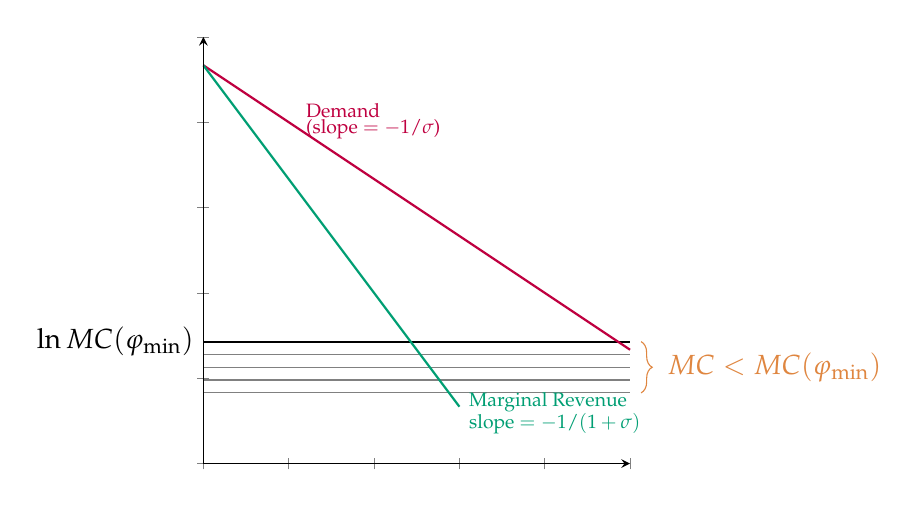
\begin{tikzpicture}
    \pgfmathsetmacro{\K}{7}
    \pgfmathsetmacro{\sigmaa}{1.5}

    \pgfmathsetmacro{\A}{7}
    \pgfmathsetmacro{\b}{0.75}
    \pgfmathsetmacro{\m}{0.35}
    \pgfmathsetmacro{\s}{2.25}
    \pgfmathsetmacro{\pmax}{\A/\b}          % choke price  (demand intercept)
    \pgfmathsetmacro{\qc}{\A - \b/\m}       % competitive quantity (P = MC)
        
    
    
    \begin{axis}[
        ymin=0, ymax=10,
        xmin=0, xmax=5,
        yticklabel=\empty,
        xticklabel=\empty,
        axis lines=left,
        enlargelimits=false,
        clip=false,
        axis on top,
        scaled x ticks=false,
        width=7cm, height=7cm,
        title style={font=\bfseries}
    ]

        
        \pgfmathsetmacro{\qs}{((\A / \b - (1/ \m  * \s) ) / ( 2/\b))}
        \pgfmathsetmacro{\ps}{ (\A / \b) - 1/\b * \qs }
        % revenue
        
        \addplot[gray, domain=0:5] {1/\m -.3};
        \addplot[gray, domain=0:5] {1/\m -.6};
        \addplot[gray, domain=0:5] {1/\m -.9};
        \addplot[gray, domain=0:5] {1/\m -1.2};

        \draw[decorate,decoration={brace,amplitude=4pt},xshift=4pt,red!75]
            (axis cs:5,1/\m) -- (axis cs:5,1/\m -1.2)
            node[midway,right=6pt]{$MC < MC(\varphi_{\min})$};

        
        
        \pgfmathsetmacro{\q}{((\A / \b - 1/ \m ) / ( 2/\b))}
        \pgfmathsetmacro{\p}{ (\A / \b) - 1/\b * \q }
        % revenue
        \addplot[black, thick, domain=0:5] {1/\m};

            %demand, rev
        \addplot[purple, thick, domain=0:5] {(\A / \b) - 1/\b * x};
        \addplot[green, thick, domain=0:3] {(\A / \b) - 2/\b * x};
            

        %\pgfmathsetmacro{\f}{\p * \q - \q / \m}
        %\addplot[blue, thick, domain=1:5] {1/\m + \f / x};

        %\addplot[gray, dashed] coordinates {(\q,1/\m + \f / \q) (0,1/\m + \f / \q)};
        %\addplot[only marks, mark=*, color=black, mark size=2pt] coordinates {(\q,1/\m + \f / \q)};


        %\node[anchor=south west] at (axis cs: 5,{1/\m+.43}) {\textcolor{blue}{Average Cost}};
        \node[anchor=south west] at (axis cs: \qs,\ps) {\scriptsize \textcolor{purple}{Demand}};
        \node[anchor=south west] at (axis cs: \qs,\ps-.5) {\scriptsize \textcolor{purple}{(slope $= - 1/\sigma$)}};
        \node[anchor=west] at (axis cs: 3,{1/(2*\m)}) {\textcolor{green}{\scriptsize Marginal Revenue}};
        \node[anchor=west] at (axis cs: 3,{1/(2*\m)-.5}) {\textcolor{green}{\scriptsize slope $= - 1/(1+\sigma)$}};

        \node[anchor=east] at (axis cs: 0,1/ \m) {$\ln  MC(\varphi_{\min})$};

    \end{axis}


    \end{tikzpicture}

 \end{frame}


\section{xxx}

\begin{frame}{Monopolistic competition}
\addtocounter{framenumber}{-1}
\centering
    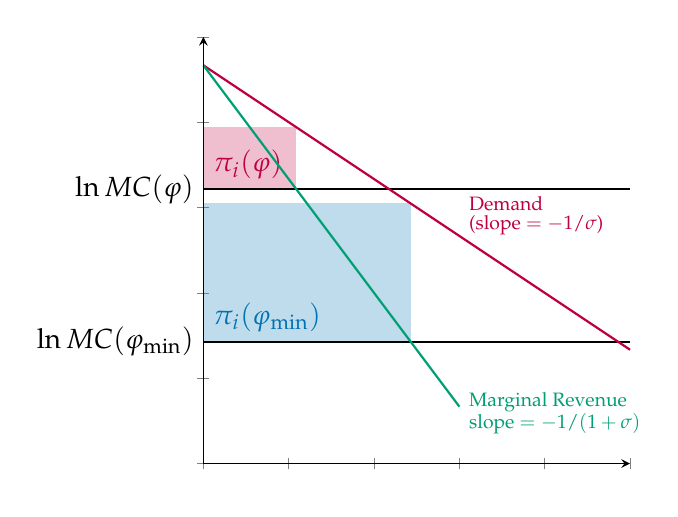
\begin{tikzpicture}
    \pgfmathsetmacro{\K}{7}
    \pgfmathsetmacro{\sigmaa}{1.5}

    \pgfmathsetmacro{\A}{7}
    \pgfmathsetmacro{\b}{0.75}
    \pgfmathsetmacro{\m}{0.35}
    \pgfmathsetmacro{\s}{2.25}
    \pgfmathsetmacro{\pmax}{\A/\b}          % choke price  (demand intercept)
    \pgfmathsetmacro{\qc}{\A - \b/\m}       % competitive quantity (P = MC)
        
    
    
    \begin{axis}[
        ymin=0, ymax=10,
        xmin=0, xmax=5,
        yticklabel=\empty,
        xticklabel=\empty,
        axis lines=left,
        enlargelimits=false,
        clip=false,
        axis on top,
        scaled x ticks=false,
        width=7cm, height=7cm,
        title style={font=\bfseries}
    ]

        
        \pgfmathsetmacro{\qs}{((\A / \b - (1/ \m  * \s) ) / ( 2/\b))}
        \pgfmathsetmacro{\ps}{ (\A / \b) - 1/\b * \qs }
        % revenue
        \addplot[fill=purple, draw=none, opacity=.25] coordinates
            {(0,1/\m*\s) (0,\ps) (\qs,\ps) (\qs,1/\m*\s)} -- cycle;
        \addplot[black, thick, domain=0:5] {1/\m * \s};
        
        \pgfmathsetmacro{\q}{((\A / \b - 1/ \m ) / ( 2/\b))}
        \pgfmathsetmacro{\p}{ (\A / \b) - 1/\b * \q }
        % revenue
        \addplot[fill=blue, draw=none, opacity=.25] coordinates
            {(0,1/\m) (0,\p) (\q,\p) (\q,1/\m)} -- cycle;
        \addplot[black, thick, domain=0:5] {1/\m};

        \node[anchor = south west] at (axis cs: 0,{1/(\m)}) {\textcolor{blue}{$\pi_i(\varphi_{\min})$}};
    
        \node[anchor = south west] at (axis cs: 0,{\s/(\m)}) {\textcolor{purple}{$\pi_i(\varphi)$}};


            %demand, rev
        \addplot[purple, thick, domain=0:5] {(\A / \b) - 1/\b * x};
        \addplot[green, thick, domain=0:3] {(\A / \b) - 2/\b * x};
            

        %\pgfmathsetmacro{\f}{\p * \q - \q / \m}
        %\addplot[blue, thick, domain=1:5] {1/\m + \f / x};

        %\addplot[gray, dashed] coordinates {(\q,1/\m + \f / \q) (0,1/\m + \f / \q)};
        %\addplot[only marks, mark=*, color=black, mark size=2pt] coordinates {(\q,1/\m + \f / \q)};


        %\node[anchor=south west] at (axis cs: 5,{1/\m+.43}) {\textcolor{blue}{Average Cost}};
        \node[anchor=west] at (axis cs: 3,\p) {\scriptsize \textcolor{purple}{Demand}};
        \node[anchor=west] at (axis cs: 3,\p-.5) {\scriptsize \textcolor{purple}{(slope $= - 1/\sigma$)}};
        \node[anchor=west] at (axis cs: 3,{1/(2*\m)}) {\textcolor{green}{\scriptsize Marginal Revenue}};
        \node[anchor=west] at (axis cs: 3,{1/(2*\m)-.5}) {\textcolor{green}{\scriptsize slope $= - 1/(1+\sigma)$}};

        \node[anchor=east] at (axis cs: 0,1/ \m) {$\ln  MC(\varphi_{\min})$};

        \node[anchor=east] at (axis cs: 0,1/ \m*\s) {$\ln  MC(\varphi)$};


    \end{axis}


    \end{tikzpicture}

 \end{frame}

\begin{frame}{Monopolistic competition}
\addtocounter{framenumber}{-1}
\centering
    \begin{tikzpicture}
    \pgfmathsetmacro{\K}{7}
    \pgfmathsetmacro{\sigmaa}{1.5}

    \pgfmathsetmacro{\A}{7}
    \pgfmathsetmacro{\b}{0.75}
    \pgfmathsetmacro{\m}{0.35}
    \pgfmathsetmacro{\s}{2.25}
    \pgfmathsetmacro{\pmax}{\A/\b}          % choke price  (demand intercept)
    \pgfmathsetmacro{\qc}{\A - \b/\m}       % competitive quantity (P = MC)
        
    
    
    \begin{axis}[
        ymin=0, ymax=10,
        xmin=0, xmax=5,
        yticklabel=\empty,
        xticklabel=\empty,
        axis lines=left,
        enlargelimits=false,
        clip=false,
        axis on top,
        scaled x ticks=false,
        width=7cm, height=7cm,
        title style={font=\bfseries}
    ]

        
        \pgfmathsetmacro{\qs}{((\A / \b - (1/ \m  * \s) ) / ( 2/\b))}
        \pgfmathsetmacro{\ps}{ (\A / \b) - 1/\b * \qs }
        % revenue
        \addplot[fill=purple, draw=none, opacity=.25] coordinates
            {(0,1/\m*\s) (0,\ps) (\qs,\ps) (\qs,1/\m*\s)} -- cycle;
        \addplot[black, think, domain=0:5] {1/\m * \s};
        
        
        \pgfmathsetmacro{\q}{((\A / \b - 1/ \m ) / ( 2/\b))}
        \pgfmathsetmacro{\p}{ (\A / \b) - 1/\b * \q }
        % revenue
        \addplot[fill=blue, draw=none, opacity=.25] coordinates
            {(0,1/\m) (0,\p) (\q,\p) (\q,1/\m)} -- cycle;
        \addplot[black, think, domain=0:5] {1/\m};

        \node[anchor = south west] at (axis cs: 0,{1/(\m)}) {\textcolor{blue}{$\pi_i(\varphi_{\min})=\bar{f}w_i$}};
    
        \node[anchor = south west] at (axis cs: 0,{\s/(\m)*1.05}) {\textcolor{purple}{$\pi_i(\varphi)$}};
        \node[anchor = south west] at (axis cs: 0,{\s/(\m)*.95}) {\textcolor{purple}{$<\bar{f}w_i$}};


            %demand, rev
        \addplot[purple, thick, domain=0:5] {(\A / \b) - 1/\b * x};
        \addplot[green, thick, domain=0:3] {(\A / \b) - 2/\b * x};
            

        %\pgfmathsetmacro{\f}{\p * \q - \q / \m}
        %\addplot[blue, thick, domain=1:5] {1/\m + \f / x};

        %\addplot[gray, dashed] coordinates {(\q,1/\m + \f / \q) (0,1/\m + \f / \q)};
        %\addplot[only marks, mark=*, color=black, mark size=2pt] coordinates {(\q,1/\m + \f / \q)};


        %\node[anchor=south west] at (axis cs: 5,{1/\m+.43}) {\textcolor{blue}{Average Cost}};
        \node[anchor=south west] at (axis cs: \qs,\ps) {\scriptsize \textcolor{purple}{Demand}};
        \node[anchor=south west] at (axis cs: \qs,\ps-.5) {\scriptsize \textcolor{purple}{(slope $= - 1/\sigma$)}};
        \node[anchor=west] at (axis cs: 3,{1/(2*\m)}) {\textcolor{green}{\scriptsize Marginal Revenue}};
        \node[anchor=west] at (axis cs: 3,{1/(2*\m)-.5}) {\textcolor{green}{\scriptsize slope $= - 1/(1+\sigma)$}};

        \node[anchor=east] at (axis cs: 0,1/ \m) {$\ln  MC(\varphi_{\min})$};

        \node[anchor=east] at (axis cs: 0,1/ \m*\s) {$\ln  MC(\varphi)$};


    \end{axis}


    \end{tikzpicture}

 \end{frame}



%----------------------------------------------------------------------%
%----------------------------------------------------------------------%


\end{document}
